

\section{Auto-complétion}
\noindent L'auto-complétion est une fonctionnalité très importante pour un IDE. Elle permet de faciliter la saisie de code en proposant des suggestions d'auto-complétion et en évitant de faire des fautes de frappe.
\newdoubleline L'auto-complétion est implémentée dans le plugin grâce à la classe "PrologCompletionContributor" qui étend la classe "CompletionContributor".

\subsection{Fonctionnement de l'auto-complétion}
\noindent L'auto-complétion est déclenchée lors de la frappe d'un caractère. Lors de l'écriture, l'auto-complétion propose les prédicats définis dans le fichier courant ainsi que dans les fichiers inclus de manière récursive.
L'arité du prédicat est également affichée dans la liste des propositions d'auto-complétion, permettant ainsi de savoir combien d'arguments le prédicat attend.
\newdoubleline Dépendamment du contexte, l'auto-complétion propose des propositions différentes. Par exemple, si l'utilisateur écrit actuellement le corps d'une règle, l'auto-complétion proposera, en plus du reste, les variables de la règle.

\subsection{Gestion des erreurs en temps réel}
\noindent Le problème que j'ai rencontré lors de l'implémention de l'auto-complétion est qu'il y a forcément des erreurs
de syntaxe dans le code, étant donné que l'utilisateur n'a pas encore fini de taper son code. Cela pose problème car
l'auto-complétion ne détecte pas les prédicats situés sous le niveau de l'erreur de syntaxe.
\newdoubleline Pour résoudre ce souci,
j'ai implémenté une méthode qui permet de détecter les erreurs de syntaxe et de les corriger en temps réel.
Cette méthode est appelée à chaque fois que l'utilisateur tape un caractère dans le fichier. Elle parcourt le fichier et
détecte les erreurs de syntaxe. Si une erreur est détectée, elle est corrigée temporairement et l'auto-complétion est relancée.
\newdoubleline Toutefois, cette méthode n'est pas parfaite car elle se limite à une seule erreur de syntaxe.

\begin{lstlisting}[language=java, caption={Méthode de correction des erreurs de syntaxe}, label={lst:correction_erreur}]
private static PsiElement removeErrorForIndexing(PsiElement rootFile) {
    PsiElement copy = rootFile.copy();
    var error = PsiTreeUtil.findChildOfType(copy, PsiErrorElement.class);

    if (error == null) {
        return copy;
    }


    var parent = error.getParent();

    boolean deleteParent = false;
    //Find all children of the parent of the error
    PsiElement lastUsable = null;
    for (var child : parent.getChildren()) {
        //If the child is an error, delete it
        if (child instanceof PsiWhiteSpace || child instanceof PsiComment) {
            continue;
        }
        if (child instanceof PsiErrorElement) {
            if (lastUsable != null) {
                lastUsable.delete();
            } else {
                deleteParent = true;
            }
            break;
        }
        lastUsable = child;
    }
    if (deleteParent) {
        if (Objects.equals(parent, copy)) {
            return null; //Impossible to delete the root file
        }
        parent.delete();
    }

    try {
        copy = PrologElementFactory.rebuildTree(copy);
        return copy;
    } catch (Exception e) {
        //More than one error in the file => impossible to rebuild the tree
        return null;
    }
}
\end{lstlisting}

\noindent Si plus d'une erreur de syntaxe est détectée, la méthode retourne null et l'auto-complétion ne se lance pas.

\subsection{Exemple d'utilisation}
\noindent Voici un exemple d'utilisation de l'auto-complétion. L'utilisateur écrit le prédicat "pred" et l'auto-complétion propose les prédicats "predicat/1" et "prediction/2".

\begin{figure}[H]
    \centering
    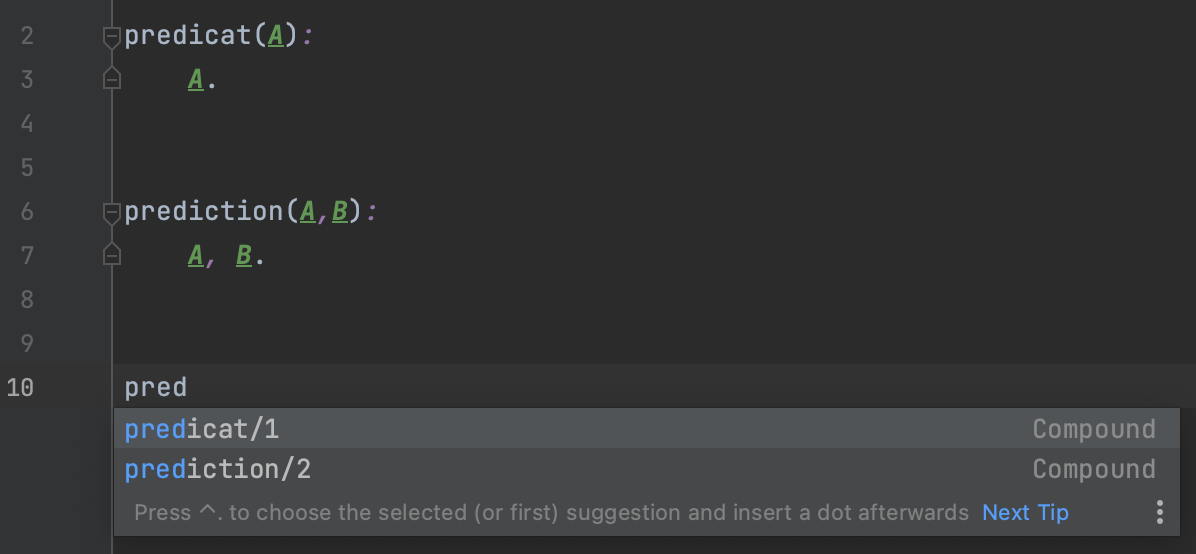
\includegraphics[width=0.8\textwidth]{images/auto_completion.png}
    \caption{Exemple d'utilisation de l'auto-complétion}
    \label{fig:auto_completion}
\end{figure}
